\documentclass[tikz,border=5mm]{standalone}

\usepackage[utf8]{inputenc}
\usepackage[T1]{fontenc}
\usepackage{xcolor}

\definecolor{accent}{HTML}{0077B6}
\definecolor{chipblue}{HTML}{0096C7}
\definecolor{chipgreen}{HTML}{00B894}

\usetikzlibrary{positioning,calc}

\usepackage{tikz}
\usetikzlibrary{positioning,calc}
\usepackage{graphicx}

\begin{document}
\begin{tikzpicture}[
	font=\sffamily,
	boardbox/.style={
		draw,
		very thick,
		rounded corners=4pt,
		minimum width=9cm,
		minimum height=2.8cm,
		align=center,
		inner sep=8pt,
		fill=accent!5
	},
	chip/.style={
		draw,
		very thick,
		rounded corners=3pt,
		minimum width=3.8cm,
		minimum height=1.5cm,
		align=center,
		inner sep=6pt
	},
	rpchip/.style={
		chip,
		fill=chipblue!10
	},
	dwmchip/.style={
		chip,
		fill=chipgreen!10
	},
	optnode/.style={
		draw,
		circle,
		inner sep=1pt,
		minimum size=0.35cm,
		fill=white,
		line width=0.6pt
	},
	labelnode/.style={
		anchor=west,
		font=\footnotesize
	}
	]
	
	% -------- Top big box: Challenger board + picture ----------
	\node[boardbox] (board) {
		\textbf{\large Challenger RP2040 UWB}\\[0.4em]
		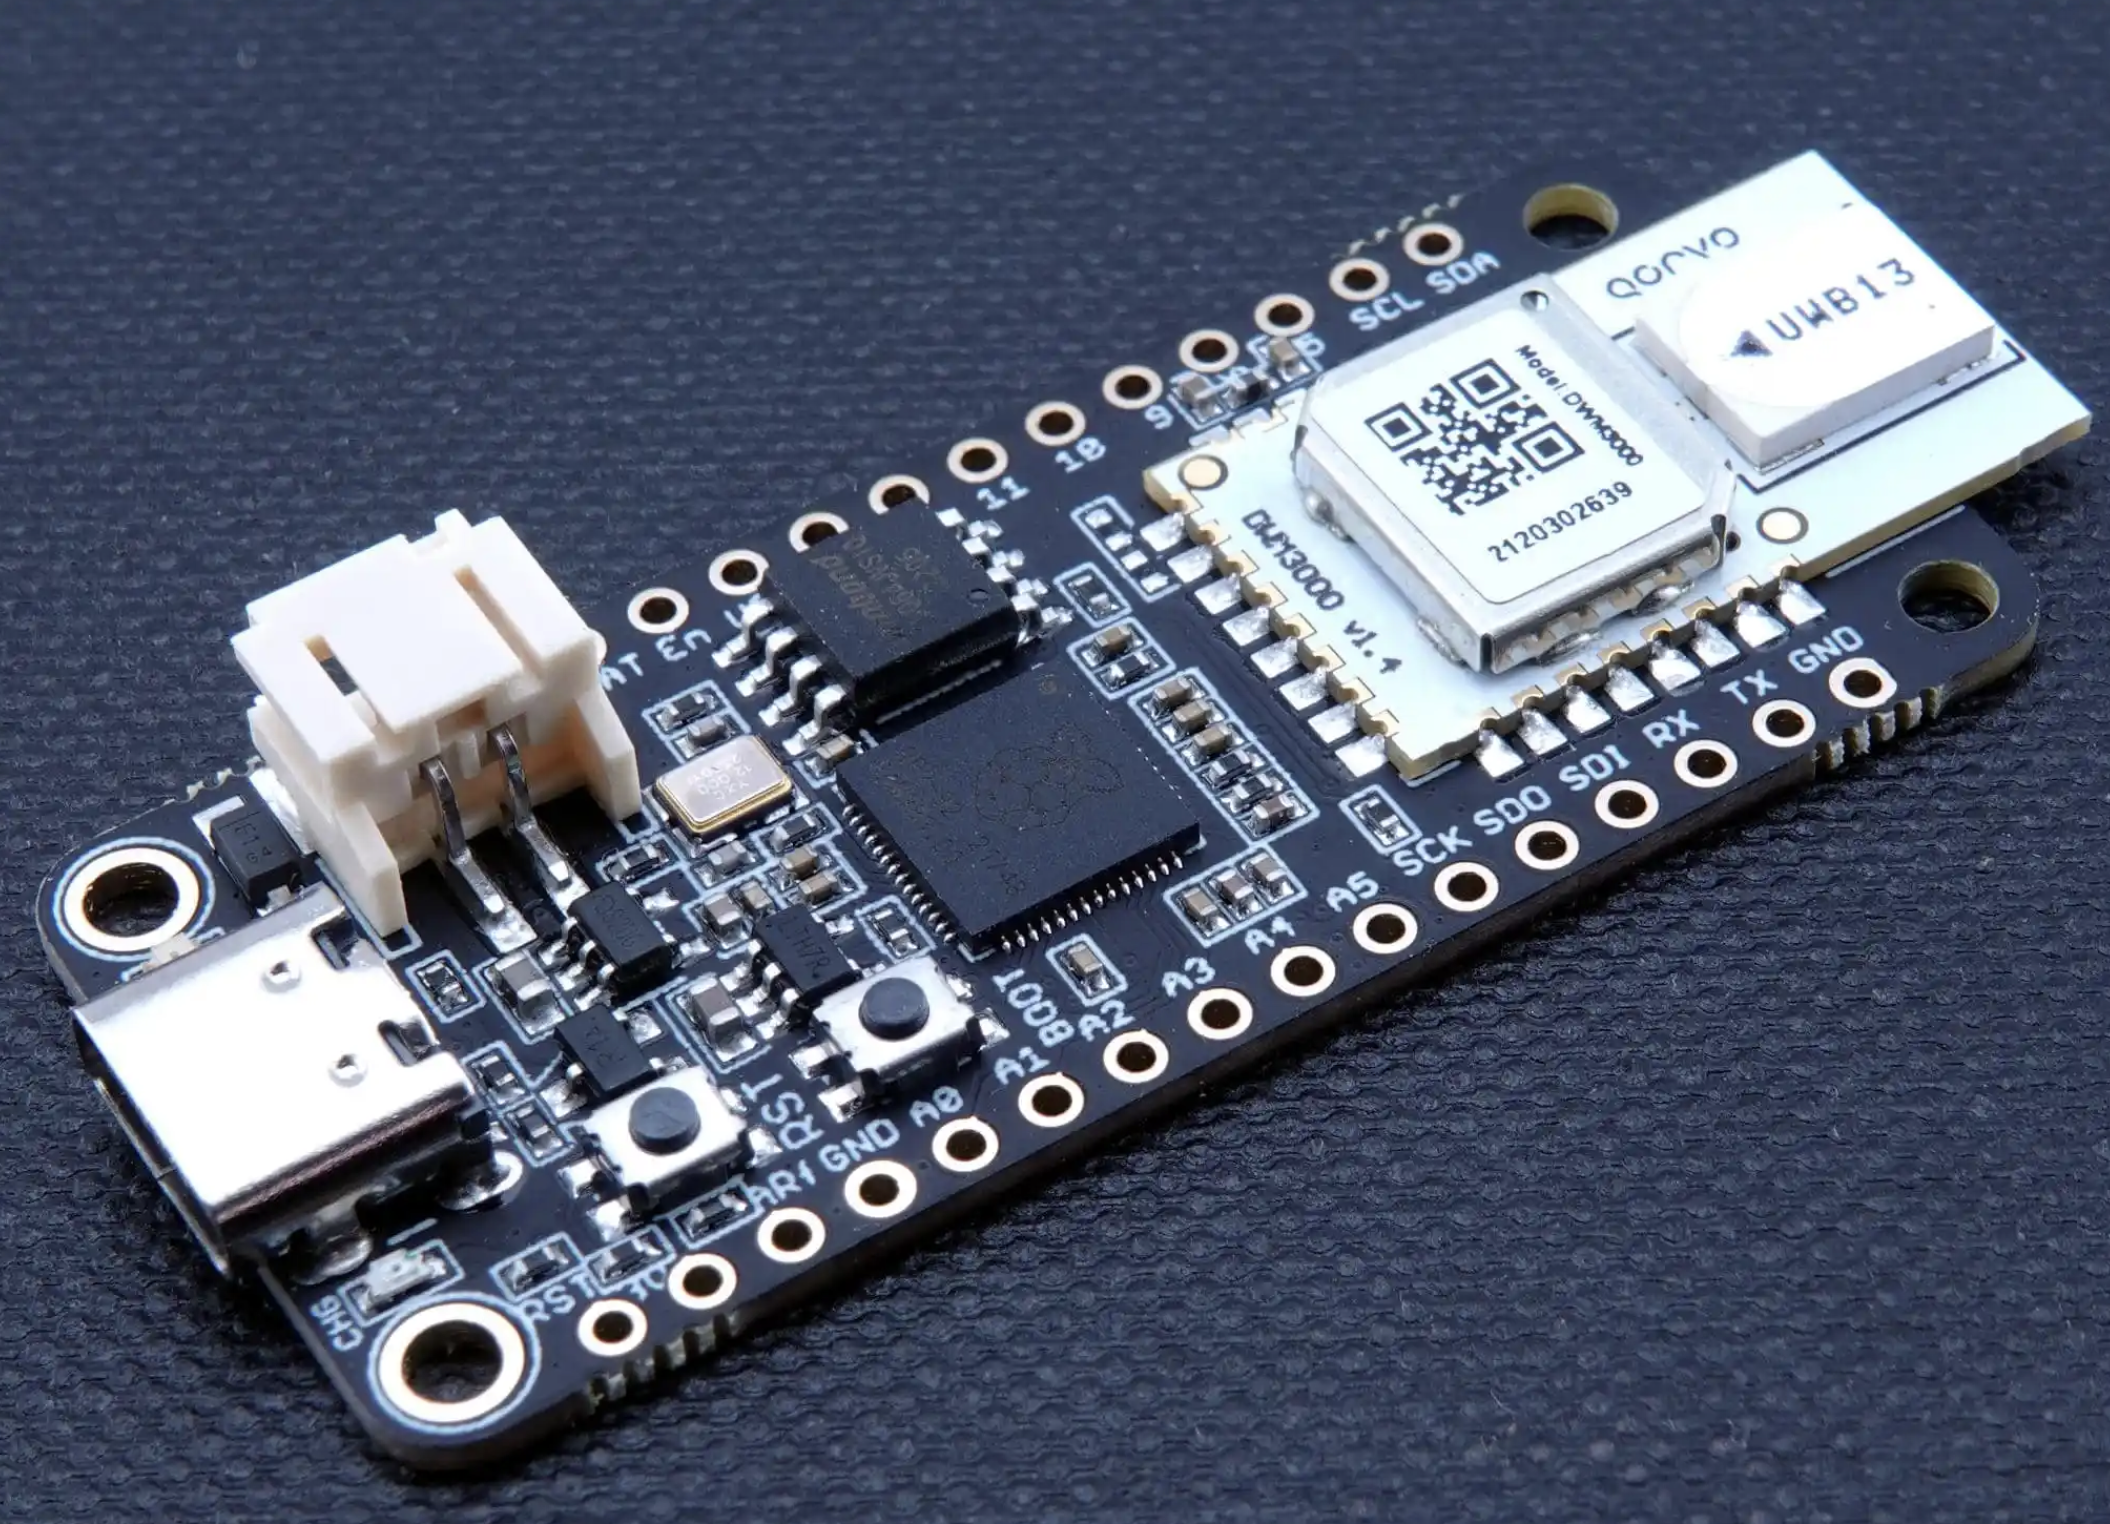
\includegraphics[width=0.\linewidth]{challenger_board}% your board image
	};
	
	% -------- Middle: RP2040 and DWM3000 "pictures" ----------
	\node[rpchip, below left=1.6cm and 0.9cm of board] (rp) {%
		\textbf{RP2040}\\\footnotesize MCU\\[0.3em]
		\includegraphics[width=0.22\linewidth]{rp2040_chip}% your RP2040 image
	};
	
	\node[dwmchip, below right=1.6cm and 0.9cm of board] (dwm) {%
		\textbf{DWM3000}\\\footnotesize UWB\\[0.3em]
		\includegraphics[width=0.1\linewidth]{dwm3000_module}% your DWM3000 image
	};
	
	% -------- Diagonal arrows from board to both chips ----------
	\draw[black,very thick,->] (board.south) -- (rp.north);
	\draw[black,very thick,->] (board.south) -- (dwm.north);
	
	% -------- Under RP2040: MicroPython / CircuitPython / Arduino ----------
	\node[optnode, below=1.0cm of rp] (microdot) {};
	\node[labelnode, right=0.15cm of microdot] {MicroPython/CircuitPython/Arduino};

	
	% simple arrow RP2040 -> top option (no extra lines through other dots)
	\draw[black,thick,->] (rp.south) -- (microdot.north);
	
	% -------- Under DWM3000: Arduino + iLabs_UWB ----------
	\node[optnode, below=1.0cm of dwm] (dwmarduinodot) {};
	\node[labelnode, right=0.15cm of dwmarduinodot]
	{Arduino + \texttt{iLabs\_UWB}};
	
	\draw[black,thick,->] (dwm.south) -- (dwmarduinodot.north);
	
\end{tikzpicture}


\end{document}
